We will define \acrfull{vr} and show the main characteristics of it through this chapter. Followed by listing a number of related projects that has been made in different places to immerse and show the user locations in different times. The last section will represent example projects that has been done in \acrshort{vr} in different places in the world focused immigration, refugees and struggles.   

\section{Virtual Reality}
In 1968 Ivan Sutherland built a \acrlong{hmd} that presented to the user left and right views of a
computer-generated 3D scene, such that when the user's head is moved, the virtual
scene remained stationary. The images were far from life like - they were simple line
drawings. But as they were stereoscopic the user perceived an impression of looking
at a solid 3D object, that was the birth of \acrlong{vr}. In 1965 he published a paper \say{the ultimate display}, that described how the computers one day will open a window for the user to the virtual world \citep{Vince2011}.  

Virtual reality is a technology which is often regarded as a natural extension to 3D computer graphics with advanced input and output devices \citep{Jayaram1997}. Ryan (2001) defined it as an “interactive, immersive experience generated by a computer” \citep{Ryan2001}. And according to G.C. Burdea and Coiffet (2017) “it is a generated computer graphics used to create a realistic-looking world that responds to the user’s input (gestures, verbal commands, etc.)” \cite[p.20]{burdea2017virtual}. Virtual reality places the users inside the experience instead of viewing a screen in front of them, the users will be immersed inside a 3D world.“The scientific community has been working in the field of virtual reality (VR) for decades, having recognized it as a very powerful human-computer interface”\cite[p.19]{burdea2017virtual}. 

As shown in Figure \ref{fig:3I} Three elements are needed to construct a virtual reality situation: immersion, interaction, and imagination. They are called the “3I’s” of virtual reality \citep{Hu2016,burdea2017virtual}.

\begin{wrapfigure}{r}{0.30\textwidth} %this figure will be at the left
    \centering
    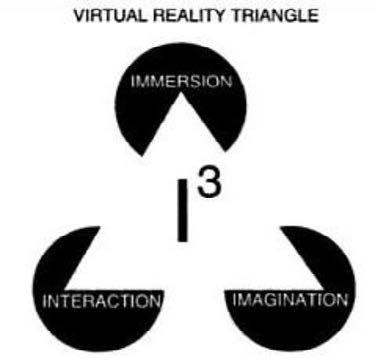
\includegraphics[width=0.30\textwidth]{3I}
    \caption{The 3I's of Virtual Reality - © 2003 by John Wiley \& Sons Inc. All rights
reserved}
    \label{fig:3I}
\end{wrapfigure}



1. \textbf{Immersion:} it is the virtual reality situation where the user feels personally inside the
scene and immerse inside the simulated virtual world.



2. \textbf{Interaction:} The interactive feedback between the user
and the virtual environment. Since it is a man-machine
interface, the system should promptly respond to the
user’s actions.




3. \textbf{Imagination:} The scene design and the construction of
the environment formulated with imagination for a
better user simulated experience.


Emotional and physical reaction would be caused to the user due to a strong mediated presence as if the virtual world existed physically, the impression of being in a real place, as well as plausibility illusion, having the sensation that the scenario being depicted is actually occurring. Those illusions occur despite the fact that the user is aware that the virtual world is only a simulation. \acrshort{vr} is one of the main trends in the evolution of presence \citep{Waterworth2014, Steinicke2016}.
The Human-computer interaction is extended from purely visual interaction to diversified interaction that the user could interact with objects in virtual reality with the perceived experiences and cognitive processing abilities as in the real world, and the feeling is close to the changes in the natural world \citep{Hu2016}.
\acrshort{vr} gives the user the ability of controlling, moving and looking in the virtual world, that gives a significant effect on the level of presence, therefore the more controlling the user would have the greater the feeling of immersion\citep{William}. \say{When we feel strong mediated presence, we react emotionally and
bodily (at least to some extent) as if the virtual world existed physically}\cite[p.4]{Waterworth2014}.


To achieve a significant immersion level for the user, we need to understand the \acrfull{fov} and the \acrfull{for} for a human. The \acrshort{fov} for a human is approximately 200 degrees with a 120 degrees of binocular overlap. The display's field of view is a measure of the angular width of a user's vision that is covered by the display at any given time as shown in Figure \ref{fig:field}. In a three-sided \acrshort{vr} projection the field of view is reduced due to the edge of the screen but it is in 100\% is the user is looking forward. However, the stereo overlap is in a larger scale at the three-sided stationary projection, some \acrlong{hmd}'s provides a 100-120 degrees of \acrshort{fov} that is a reasonable portion of the human visual rang. Although the stereo overlap is very important and that can vary in \acrshort{hmd}'s where the two displays are more of less widely separated, if the overlapping  
\acrshort{fov} for both eyes is as small as 30 degrees, it will be difficult to perceive stereopsis \citep{William}.
If we move towards an object, the ciliary muscles adjust the shape of the lens to accommodate
the incoming light waves to maintain an in-focus image. Also, the eyes automatically
converge to ensure that the refracted images fall upon similar areas of the
two retinas. This process of mapping an image into corresponding positions upon the
two retinas is the basis of stereoscopic vision. The difference between the retinal images
is called binocular disparity and is used to estimate depth, and ultimately gives rise to
the sense of three dimensional\citep{Vince2011}.

\begin{figure}[ht]
    \centering
    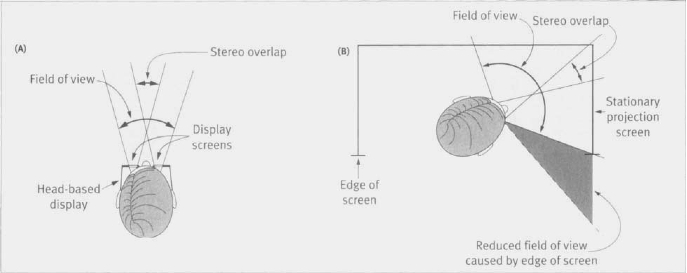
\includegraphics[width=0.90\textwidth]{Fod.png}
    \caption{Field of View - \citep{William}}
    \label{fig:field}
\end{figure}


\begin{figure}[ht]
    \centering
    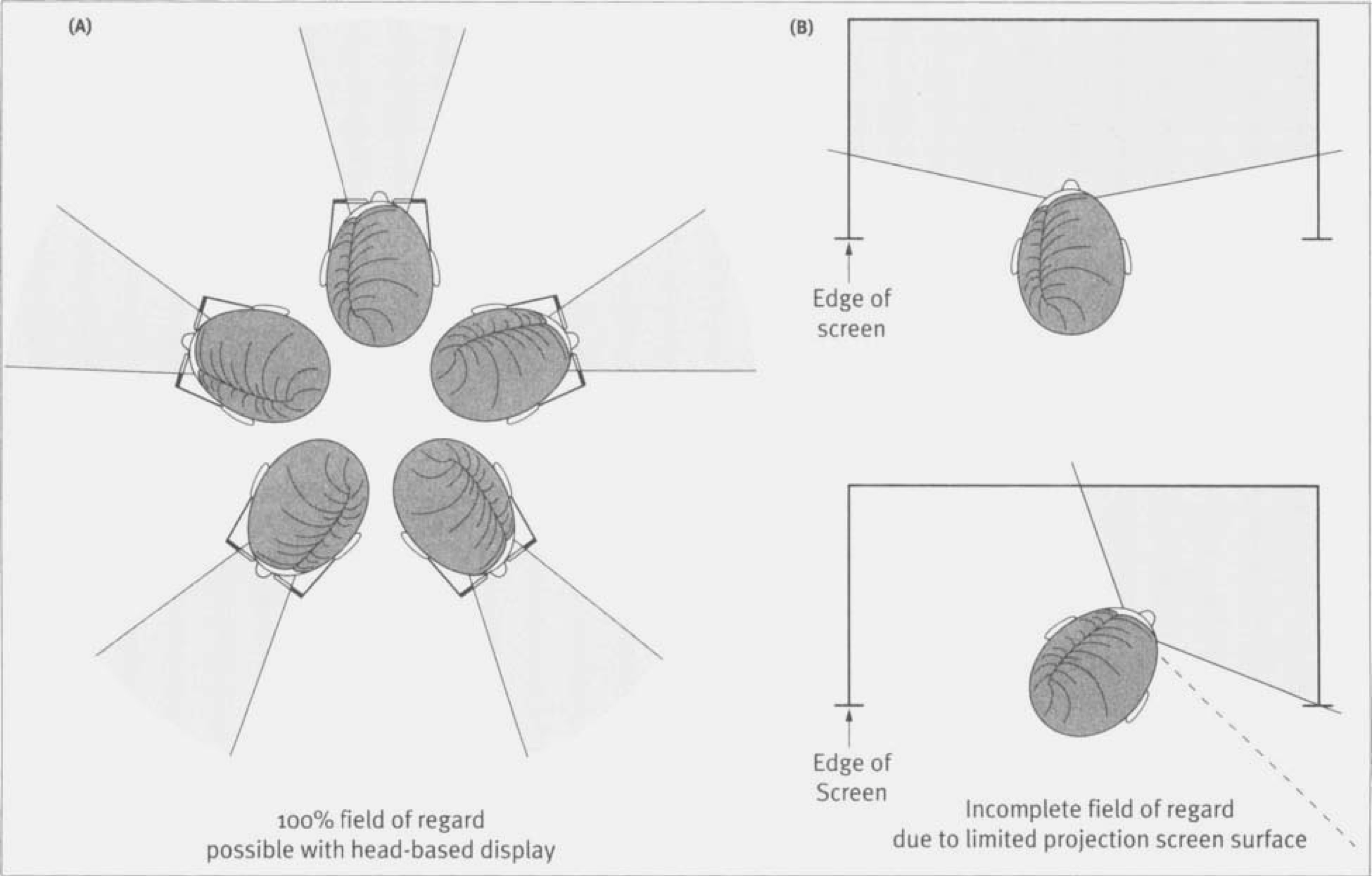
\includegraphics[width=0.90\textwidth]{fov.png}
    \caption{Field of Range - \citep{William}}
    \label{fig:fod}
\end{figure}

The \acrfull{for} is the amount of space that is surrounding the user inside the virtual world. As displayed in Figure \ref{fig:fod}, the \acrshort{for} in the \acrshort{hmd} is 100\% due to the screens that always face the user's eyes, regardless for the direction that the user will look at, the virtual world will always be in front of his eyes. The \acrshort{for} is usually less than 100\% in the three-sided \acrshort{vr} projection because the virtual world will always need screens and it not dynamic in movement as the \acrlong{hmd} \citep{William}.

A \acrshort{hmd} is nothing more than a stereoscope, it doesn't use only photographs but also animated
video images. What is essential though, is that the views seen by the two eyes
must overlap and it is in this area of overlap that stereoscopic vision is perceived \citep{Vince2011}.
Figure \ref{fig:field} presents this stereo-overlap area. As the two images are taken from two different positions in space, the brain uses these
differences to create a single image that contains depth information \citep{Vince2011}. Therefore, the use of \acrshort{hmd}'s would have its consequences, for instance a low-latency tracking "not more than 2ms (millisecond)" is desired to adapt the display imagery to the physical movement of the viewer, also to avoid motion sickness since large latency's have serious negative effects on the simulation, for example, headaches, nausea, or vertigo \citep{burdea2017virtual, Vince2011, Steinicke2016}.

A technological revolution was made by smartphones where they combined between communication and computation devices, where they are small by size and can fit in the user pocket. the high computation processing in the smartphones allowed is enough to process \acrshort{vr} environment, therefore it enabled a light-weighted and practical \acrshort{vr} devices and the resurgence of the internet in \acrshort{vr}. 



\begin{figure}[ht]
    \centering
    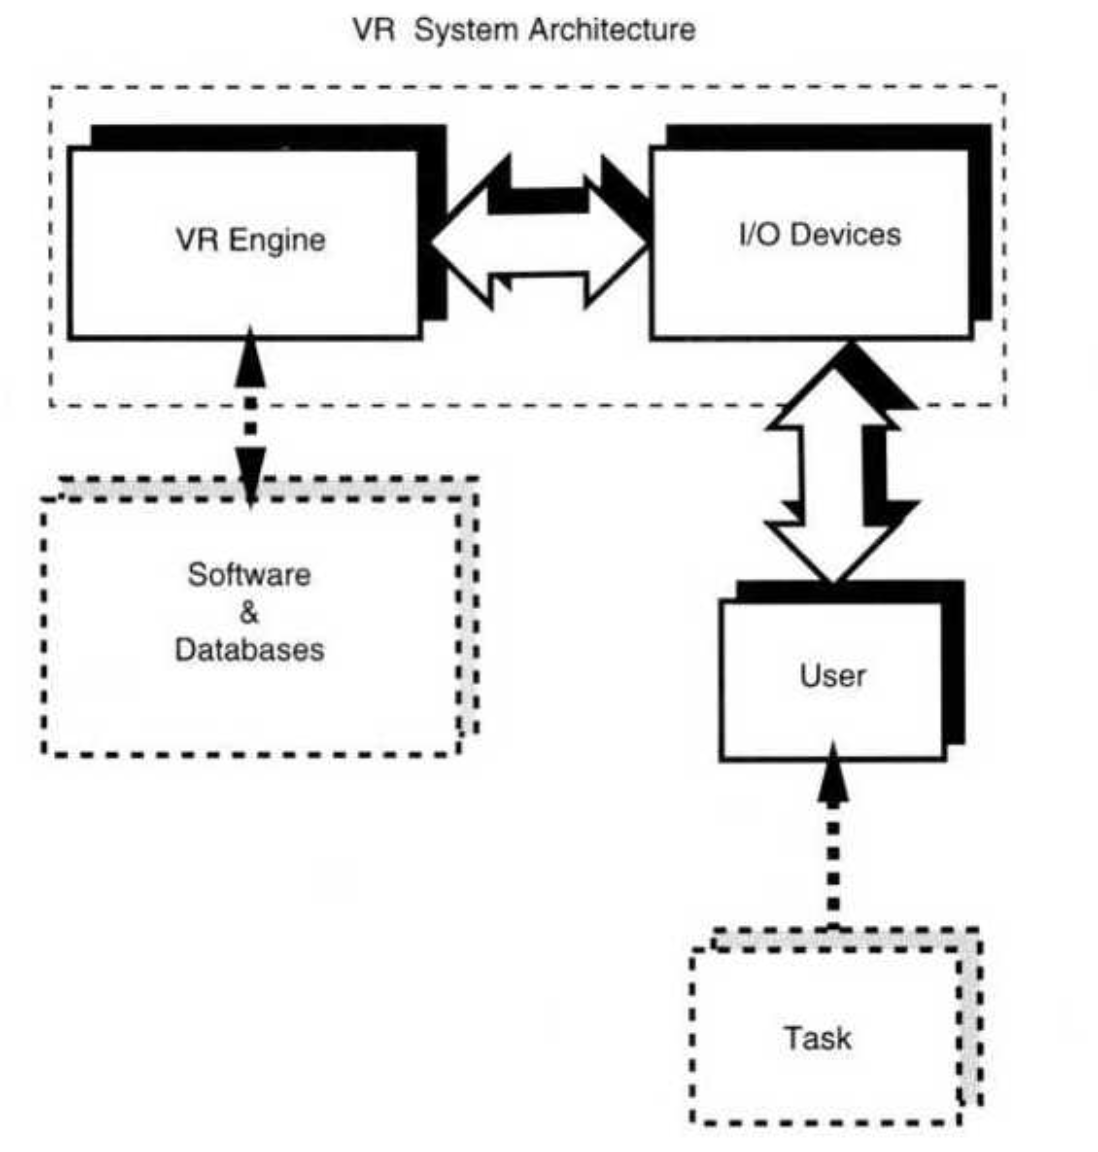
\includegraphics[width=0.50\textwidth]{images/VR.png}
    \caption{a nice plot}
    \label{fig:mesh1}
\end{figure}




The classical five components of a \acrshort{vr} system are:
\begin{itemize}
  \item Software and Database
  \item VR Engine
  \item I/O Devices
  \item User
  \item Task
\end{itemize}


\subsection{Software and Database}


 \acrshort{hmd} is nothing more than a stereoscope, it doesn't use only photographs but also animated
video images. What is essential though, is that the views seen by the two eyes
must overlap and it is in this area of overlap that stereoscopic vision is perceived \citep{Vince2011}.
Figure \ref{fig:field} presents this stereo-overlap area. As the two images are taken from two different positions in space, the brain uses these
differences to create a single image that contains depth information \citep{Vince2011}. Therefore, the use of \acrshort{hmd}'s would have its consequences, for instance a low-latency tracking "not more than 2ms (millisecond)" is desired to adapt the display imagery to the physical movement of the viewer, also to avoid motion sickness since large latency's have serious negative effects on the simulation, for example, headaches, nausea, or vertigo \citep{burdea2017virtual, Vince2011, Steinicke2016}.




  
\section{Related Work}
The SCULPTEUR project – Semantic and content-based multimedia exploitation for European benefit – is developing a solution for museums to create and manipulate digital representations of museum objects. SCULPTEUR utilizes multi- stereo and silhouette techniques to create 3D museum object reconstructions stored in a database together with other multimedia data. The project is also aimed at developing a semantic layer providing a variety of search and content analysis opportunities. Moreover, the system gives users seamless access to the distributed databases of cultural data by offering a set of tools encompassing educational software products [SCULPTEUR 2003].
The 3D Murale project – 3D Measurement and Virtual Reconstruction of Ancient Lost Worlds of Europe – is aimed at developing a system capable of recording archaeology excavation phases using Virtual Reality techniques. In addition to the artifacts also stratigraphical layers can be modeled. This requires utilizing diverse 3D capture techniques. Furthermore, the project offers the reconstruction of excavated remains of pottery, sculptures and buildings as well as their visualization in a way as they possibly looked like throughout ages [3D Murale 2003].
In recent research on exploitation of modern technologies in cultural heritage, an increasing role of Augmented Reality can be observed. A notable example is the ARCHEOGUIDE project intended to develop a wearable AR tour guide at cultural heritage sites [ARCHEOGUIDE 2003]. ARCHEOGUIDE allows visitors to see virtual reconstructions of ancient buildings. A user is equipped with a see-through Head-Mounted Display (HMD) and wearable computing equipment. The equipment is responsible for visualization of appropriate information on the HMD depending on the visitor’s position and orientation in the site. Similar to ARCHEOGUIDE in terms of applied technology is the LIFEPLUS project. A fundamental difference is the presented contents that in case of LIFEPLUS additionally encompass real- time 3D simulations of ancient fauna and flora [LIFEPLUS 2003].
Another example of an outdoor solution is the Ename 974 project aimed at virtual reconstruction of an extensive archaeological site located at Ename, Belgium [Ename 974 2003]. Visitors are offered with virtual reconstruction of early-medieval buildings in stationary AR kiosks. Users can see visualizations of virtual models overlaid on video data captured by a camera. Using touch screen displays they can control the camera and the displayed data.
Another group of systems exploiting AR techniques to visualize cultural heritage encompasses indoor applications. An example of such a system is the Virtual Dig Experience installed in the Seattle Art Museum [Virtual Dig 2003]. Using VR and AR techniques visitors, particularly children, can discover artifacts for themselves. Users are presented not only with the artifacts but also with their archaeological context. Real objects such as brushes and small shovels are used for user interaction. The Virtual Dig has been developed based on the HI-SPACE [HI- SPACE 2003] and ARToolKit [ARToolKit 2003] packages.
The Virtual Showcase project [Bimber et al. 2003; Virtual Showcases 2003] is intended to eliminate the necessity of using unusual methods of presenting cultural objects, which is one of the weaknesses of most VR and AR systems. The project aims at integrating the AR technology into a traditional museum showcase format. Virtual images can be projected on the sides of a specially designed showcase allowing users to explore both the real objects and their virtual representations.
\citep{Rahaman2011InterpretingPerspective}

\section{Example projects}
\textbf{Auschwitz Virtual Tour}\footnote{Auschwitz VR Tour-\url{https://youtu.be/EOM_CxAKB_Y}}: The German broadcasting institution WDR made a 360$^{\circ}$
documentary in Auschwitz concentration camp. Within the documentary, some Holocaust
survivors tell their stories. While listening to the stories and seeing the different locations in
the camp the user could feel the fear and horror that people suffered from. The video
immerses the user through the sound of the surrounding environment in the camp, you can
hear the wind and the sound gives a slight feeling of the cold weather over there. The
experience is immersive, but there is no interactivity with the user.


\textbf{Clouds over Sidra}\footnote{The Za’atari camp VR Tour-\url{https://youtu.be/mUosdCQsMkM}}: A 12 years old girls’ daily life story at the Za’atari refugee camp in Jordan
showed in virtual reality. The camp is a home for 80,000 Syrian refugees, half of them are
children(“Syrian Refugee Crisis – UN Virtual Reality,” 2015). The documentary was made by
the United Nation to raise awareness about the Syrian crisis. The video contained a number
of short videos from different parts of the camp, and it’s being synchronized while Sidra
narrates her story. It is more like watching a video with empathy than being immersed, but
the video presents the real life of the camp. Although the difference that while watching and
listening to the story, the user observes the people how they actually survive and live in the
camp. Therefore, the user does not have to imagine how is life over there.


\textbf{Carne y arena}\footnote{Carne y Arena Trailer-\url{https://youtu.be/zF-focK30WE}} : A highly professional
Virtual reality project that puts viewers
into the harsh life of an immigrant. The
user is placed among a group of
Mexican immigrants passing the
borders into the U.S. It was written and
directed by Alejandro G. Iñárritu. It Is a
full virtual reality experience; the user
needs to reserve an individual session
on the website. According to Pinotti (2017) you go in a dark room; your feet are on the sand (coarse grain, rough feeling) then, two assistants welcome you and provide you with the
necessary devices: an Oculus Rift headset, a backpack connected via cables to a powerful
computer and you are ready to be caught up in a nightmare \citep{Pinotti2017}. The project is
subtitled by ‘Virtually present, Physically invisible’. Pinotti (2017) defined, Virtually present:
“you are transported in the middle of the desert, among men, women, and children who try
their voyage of hope”. Physically invisible: “you are present, but nobody sees you and after a
while, you start to feel the need to be noticed and seek acknowledgment of social
recognition” \citep{Pinotti2017}. The project was developed with high technology, like 3D
modeling, visual effects, sound. The interaction of the user and the feeling of “being there”
by placing the user in a special environment, leads to a unique experience of immersion.


